%!TEX root=main.tex

% ========
\section{SM-EFT: The Bottom-Up Approach}
\label{sec:classification}

Currently, in particle physics, there are no experimental
results that would allow one to clearly identify or completely rule out any of the 2499 additional possible
dimension-six operators
(see Sec.~\ref{sec:eftintro}) as a signal of BSM physics. 
\PMnote{As we will discuss, the SM-EFT approach is used by physicists' in different stages.
These three stages are used to support the search for BSM both experimentally and theoretical,
with several goals coming together: they serve as accounting scheme both in general and in a
focussed approach on a special sector of the SM. 
They therefore set constraints on model building and, in case of an indication for a non-vanishing
Wilson coefficient, allow physicists to evaluate potential general consequences and possible 
realizations in a concrete BSM model.}

We refer to \emph{Stage 1} \PMnote{the SM-EFT with all 2499 operators.}
%In this situation, choosing
%a value for a particular set of coefficients $c_i$ would predict a
%certain observable signal.  It can thus be falsified for such a
%particular choice, if the deviation is not found. Assuming one
%individual $c_i~\neq$ 0 would represent one new vertex between SM
%particles, and thus would represent a \emph{specific} target. This can
%be compared to the Fermi theory, which represents a direct vertex
%between 4 SM fermions. Likewise, a subset of several coefficients
%$c_i~\neq$ 0 would represent a set of several new vertices between SM
%particles.
Globally, the SM-EFT does not represent a specific new interaction
and thus it has no experimental target in a sense that would allow it to
guide experimental searches.  If all coefficients 
$c_i$ in Eq.~\ref{eq:smeft}
were considered to be potentially nonzero, it would mean that all
distributions of a wide variety of experimental observables could
differ in a wide variety of possible ways from the SM prediction.
Thus, to say that the SM-EFT at Stage 1 is a
good description of physics beyond the SM is only to say that in some
sector of particle physics some measurement of some interaction (be it
in the form of an interaction rate, an asymmetry, a kinematic
distribution or any other type of possible particle physics
measurement) between SM particles is measured to be different from
the SM, and that this deviation is consistent with the non-observation
of a new resonance and that the underlying physics obeys all SM
symmetries. 
Such a framework effectively allows an extremely wide variety
of deviations from the SM in all areas of particle physics, without
any specific theoretical preference of what should be experimentally
expected in a new measurement. We consider this as not being a
useful concept for an experimental target. In consequence, we also doubt the
representational character of the global SM-EFT. It does not represent any physics beyond the SM, it just serves as a tool to
parametrize the size of possible deviations from the SM which are
consistent with the underlying assumptions of the SM-EFT. Therefore,
we propose that under the experimental status of Stage 1, the SM-EFT does
not possess the characteristics of a model, as outlined in
Section~\ref{sec:models}, but instead should be regarded as a
parametrisation of the available room for deviations from SM
predictions.

\PMnote{We now turn to what we consider \emph{Stage 2} of the bottom-up approach.
Since it is impossible to control
2499 parameters and the corresponding experimental distributions
simultaneously---both in the experimental and theoretical
sense, physicists typically just focus on a small subset of the SM-EFT and attempt to
include all relevant experimental information from one well defined
experimental sector. 
Parts of the SM-EFT can be applied separately to top physics, or bottom
physics (see Section~\ref{sec:Bphysics} for an example), or vector boson
self-interactions or fermion pair production, or Higgs physics. 
Fundamentally, such separations between different sectors of the SM
are not strictly valid. The freedom of choice of the basis of the
SM-EFT (see Section~\ref{sec:smeftphysics}) makes it a matter of
choice which experimental sectors are connected through the structure
of the SM-EFT operators.}

\PMnote{Since the strongest focus during the past years, was and is on Higgs physics, as a new
and unique potential portal for new physics, let us clarify the stage 2 concept with
this example~\citep{Espinosa:2016ovf}.
The number of operators for such dedicated studies are given by a suitable choice
of the basis, experimental constraints on the corresponding Wilson coefficients and
possibly assuming additional symmetries.
For example, assuming no additional source of CP violation and assuming
only flavour-diagonal couplings reduces the number of coefficients to
59~\citep{Buchmuller:1985jz,Grzadkowski:2010es}, 
which still far exceeds the experimental capabilities for setting
constraints from separate experimental sectors. 
However, measurements already put significant constraints on several of these
such that for experimental and theoretical treatments only six are considered
relevant.
This reduction to a
few parameters is operationally motivated and makes \emph{Stage 2} experimentally and
phenomenologically useful by mapping measurements to a manageable set
of parameters. Epistemic,
pragmatic, and experimental values, such as experimental accuracy,
novelty of access to a phenomenon, and sensitivity of a measurement to
a specific set of SM-EFT operators may play a role in choosing a
certain sector at a time. Therefore, it is predominantly just an
operational step. } 

Further, this sectorised SM-EFT still lacks a specific target of representation and thus a key characteristic of being a model. 
This conclusion is also
supported by the current experimental constraints of the SM-EFT Wilson
coefficients in the Higgs boson sector: for a model with a clear
experimental target, one would expect that experimental results allow one
to constrain the allowed range of parameters or to refute the
model. However, as present results show~\citep{ATL-PHYS-PUB-2019-042},
the SM-EFT parameters cannot be constrained if more than two Wilson
coefficients are tested at the same time: there are ``flat
directions'' for all parameters, which means that effectively every
parameter can take any value. Therefore, it carries no
\emph{specific} information based on the data.

This changes if specific operators are selected, either by
experimental indications or even undisputed experimental evidence of a
new signal, or by dedicated additional theoretical motivations beyond
the logic of the SM-EFT. Once such additional experimental evidence or
theoretical background is used to constrain the SM-EFT, we refer to it
as \emph{Stage 3} SM-EFT.  In such a situation, only a very small set
of SM-EFT operators would be considered to be non-zero, either due to
additional symmetries invoked by a concrete model of New Physics, or
because an experimental signal of physics beyond the SM favours a
dedicated basis and allows to measure a non-zero value for a small set
of operators in this basis at a statistically
significant level. An example for a possible emergence of such a
situation is given in Section~\ref{sec:BphysicsConcepts}.

In this case, it would be possible to meaningfully reduce the
ambiguities in representation stemming from the different bases. The
most efficient SM-EFT basis that describes the data with the
smallest set of operators would then represent a small subset of the
possible new effective vertices.  This is not dissimilar to the
development of the Fermi theory (see~\ref{ssec:Fermi}). In the Fermi
theory, one 4-point interaction vertex with one associated coefficient
$c^2=G_F$ is added to the previously known physics in an effective
theory. In case of the bottom physics analyses described in Section~\ref{sec:BphysicsConcepts}, the apparent
violation of lepton-flavour unification in the bottom sector motivates
the use of specific operators to describe observed experimental
features, thus they represent specific interactions. This is a
qualitative difference in Stage 3 with respect to Stage~2: the SM-EFT
no longer describes potential non-resonant deviations from the
SM in a non-unique way (as in Stage~2), but in Stage~3 one selected basis of
the SM-EFT uniquely describes (observed or expected through an
underlying concrete model of New Physics) experimental features that
are distinctively different from the SM.

% =======
\subsection{Differences between these Stages}

Let us illustrate the differences 
{\PMnote{between these stages} in more detail. 
\MSnote{Given that our main focus is whether and at what stage SM-EFT can be considered as a model, we will especially focus on the difference between stages 1 and 3. Stage 2 can be considered as a practically motivated restriction of of the full SM-EFT focusing on specific sectors of the SM or specific types of processes. The concrete implementation of a stage 2 analysis will always be executed in terms of a large variety of stage 3 analyses. \emph{(Check if this works because we had to better define the differences and so we cannot simply leave it out because otherwise the referee asks why not just two stages.)}} 

The first point to notice is the different practice of physicists already discussed in
Sect.~\ref{sec:physrepres}.
SM-EFTs work as an accounting scheme to be able to quantify constraints on, or deviations
from SM distributions and possibly correlate different operators.
As such the SM-EFT is a convenient tool to globally assess the status of the SM.
In contrast, as exemplified in the next Section, using a current discussion in particle physics,
selecting one or a few operators is a standard procedure to assess potential BSM physics.
Such selection is based on a general idea, as for example~\cite{Weinberg:1979sa} for lepton
and baryon number violation, or \cite{Eichten:1983hw} for fermion sub--structures, the
selection might however also be suggested by indications from measurements. 
As the quotes by physicists in Sect.~\ref{sec:physrepres} show, measuring the Wilson coefficients
are tools for BSM models that are of interest to physicists.
Virtually no physicist considers all SM-EFT operators to simultaneously be indicative for BSM. 

This practical aspect of the different stages has epistemic reasons that we use in the discussion of
the model character.
While a selected operator provides a target for further theoretical and experimental studies,
the SM-EFT as a whole does not provide such.
For example,~\cite{Weinberg:1979sa} uses the B--L non--conserving operators as general
constraints for B--L violation that should be understood better by 'specific gauge models of
baryon decay' (1569).
Experimentally, in such a case the target would be the search for proton decay.
For a current example we again refer to Sect.~\ref{sec:BphysicsConcepts}.
In contrast, SM-EFT does not provide any target:
as for which BSM effects may be observed, it replies by 'possibly in any deviation from the SM'
-- something that is known before.
Again, we emphasize that this does not mean SM-EFT is useless, it quantifies deviations.

The absence, respectively existence of a target has repercussions for the testability of
SM-EFT as a whole or for a single operator.
The first point to note is that testability in either case is not well defined without
further assumptions.
For example, if Weinberg states that the dimension 5 operator would produce neutrino masses
between 10$^{-5}$ and 10$^{-1}$ he assumes certain Wilson coefficients: a cut--off scale of 
10$^{14}$ GeV, suggesting GUTs, and a coupling of $\cal{O}$(1).
Thus the EFT \textit{simpliciter} does point out at most possibilities. 
To provide a quantitative
and testable statement it has to be supplemented by an additional assumption that comes
closer to a concrete model.
Comparing SM-EFT in total and one selected operator, one immediately sees that it is
virtually impossible to derive meaningful predictions for 2499 Wilson coefficients, but,
based on a general idea about underlying physics processes, very well possible for 
a dedicated operator.
In consequence, the SM-EFT cannot be tested in a meaningful sense, a single operator however can. 
  
\sout{The final point we want to make is the representational content of SM-EFT vs. a single
operator.
We assume a representation of an object A in a theory/model B to have at least one 
or a few (measured or measurable) properties of A to be formally included in B.
\textbf{Needs a philosophically more correct definition}.
Representation of something thus requires a target to be represented.
Since we discussed before that SM-EFT lacks such a target, it also has no representational
value, different to a single selected operator.
This may at the first glance seems strange if SM-EFT is just considered as a virtually
infinite collection of single operators. 
As such it requires a loss of representation by proceeding from one and an infinite number of operators.
Beyond the arguments given above, let us note that such a loss of quality is not unusual
in such an expansion.
Assume a homogeneous plane. 
While a direction is given by selecting a certain angle, no direction is given by allowing for
all angles.}\MSnote{I think we will provide this analysis in Section 7. The following paragraph is pretty homeless here and I suggest moving it before 5.1.}

We want to remark that these stages are meant conceptually but not necessarily temporally.
Indeed, as an example, in the early 1980s, without reference to
a systematic development of the SM-EFT,~\citep{Eichten:1983hw} proposed,
a model for fermion substructure ('preons') in analogy to the Fermi theory.
% These considerations imply that the status of an EFT as
% a model cannot be answered just by looking at a Lagrangian. 
%For example, experimental findings or theoretical assumption on the underlying physics
% may imply a concrete representational property of a selection of operators.
% In the following section, an example of an evolving interpretation of a set of statistically partially significant measurements of deviations from the SM in a Stage~3 SM-EFT is given.

 % ===========
\section{Exemplifying Search Concepts in Bottom Physics}\label{sec:BphysicsConcepts}

In Section~\ref{sec:classification}, we discussed a classification
scheme for the SM-EFT, where the experimental status of the theory can
play an important role in the reduction of very many degrees of
freedom to a very small number. The SM-EFT in \emph{stage~3} thus can
gain representative character through the identification of new
vertices beyond the SM, which represent new types of interactions
between SM particles. One such experimental situation, which has been
emerging over the last years, are precision tests of rare leptonic
decays of $B$ mesons, where lepton universality is
% violated~\citep{Buttazzo:2017ixm} in
% experiments~\citep{Aaij:2019wad,Abdesselam:2019wac,Aaij:2017vbb,Aaij:2015oid,Abdesselam:2019dgh}
violated in experiments
at a statistical significance of around ${\cal O}(3\,\sigma)$ on
average for sensitive single measurements \citep{Aaij:2015oid,Aaij:2017vbb,Aaij:2019wad,Abdesselam:2019dgh,Abdesselam:2019wac,Buttazzo:2017ixm}.
In this section, it is shown how the different BSM approaches are applied to this heavily discussed set of physics processes.

In the SM, the electroweak gauge bosons, $Z$ and $W^\pm$, couple to
the three lepton flavours ($e$, $\mu$, $\tau$) universally (i.e.\ with
the same strength).  Recent measurements of B-meson decays such as
$b \to sl^+l^-$ and $b \to c l \nu$ show hints for the violation of
lepton flavour universality (LFV) (for an overview, see
also~\citep{Albrecht:2018frt}).  As of yet the statistical and systematic
uncertainties are too high to allow firm claims, but if confirmed,
these measurements would provide evidence for BSM physics. To evaluate
LFV, the three approaches introduced in
Section~\ref{sec:eftintro} to evaluate LFV are pursued: concrete
models; Stage~2 and Stage~3 EFTs; and
simplified models. 

% ========
\subsection{Concrete BSM Models}
\label{sec:B-con-BSM}

To explain the apparent LFV with a concrete model, new particles with
different couplings to leptons are assumed.  Furthermore, since LFV
has only been observed for the bottom quark, it is suggestive to
assume such a particle to have an affinity to bottom quarks, or in
general to quarks of the third generation.  Attempts to explain the B
anomaly include SUSY~\citep{Altmannshofer:2017poe}, strongly
coupled models, such as composite Higgs~\citep{Greljo:2015mma}, or
additional (heavy) Z's or W's~\citep{Boucenna:2016qad}.

While these models may be easily adjustable to work for LFV in 
bottom hadron decays, they also have implications for other processes
that cannot be accommodated easily and require a high level of fine
tuning. Furthermore, some of these hypotheses, although starting from
a different underlying concept, arrive at a similar phenomenology for 
LFV effects, and thus cannot be experimentally distinguished from each other. Therefore, physicists currently turn to EFTs and simplified models, which
provide general constraints on a viable model, %to guide building a viable model,
despite the fact that concrete models would have been more satisfying.
This is why several authors prefer a bottom-up approach using the
SM-EFT (see e.g.~\citet{Buttazzo:2017ixm}).

% ==========
\subsection{B-physics Anomalies: Effective Field Theory Approach}\label{sec:Bphysics}

The physics of bottom hadrons involves different scales, the QCD scale of
some 100 MeV, the scale of the bottom quark of some 4 GeV and the
electroweak scale of some 100 GeV. It is thus adequate to use an EFT to
describe bottom decays.  The corresponding Lagrangian, containing only
transitions of the bottom quark into other SM particles, is a subset
of the SM-EFT and has been used in analyses of bottom decays and
transitions for some 20 years.

While the indication of LFV can be analysed with a full EFT for bottom
quarks, the observed properties indicate only certain operators to be
relevant as pointed out in~ \citet{Buttazzo:2017ixm}. Conveniently the
(potential) BSM effects can be represented as an additional
contribution to the SM Lagrangian.  For example in
\citet{Buttazzo:2017ixm} the effective Lagrangian for
$b\rightarrow s l^+l^-$
\begin{equation}\label{eq:leff}
{\cal L}_{\rm eff} = {\cal L}_{\rm SM} - \frac{1}{v^2}\lambda^q_{ij}\lambda^l_{\alpha\beta}\left[C_T(\overline{s}^i_L\gamma_\mu\sigma^a b^j_L)(\overline{e}_L^\alpha\gamma^\mu\sigma^a e_L^\beta)+C_S(\overline{s}_L^i\gamma_\mu b_L^j)(\overline{e}_L^\alpha\gamma^\mu e_L^\beta)\right]
\end{equation}
is postulated for the production of $e^+,~e^-$ (or $\mu^+ \mu^-$ by
replacing $e_L$ by $\mu_L$).\footnote{Instead of general quark
  transitions, here only the one relevant for the indication of LFV,
  namely the $b\rightarrow s$ transition is used} It contains two
four-fermion operators which describe new interactions between
left-chiral quark and lepton fields $(s,b)_L$ and $(e,\mu )_L$,
respectively, already basically known from Fermi theory.  The
coefficients $C_T$ and $C_S$ are flavour blind and encode the new
physics scale $C_{T,S} \propto \ v^2/\Lambda^2$, where $v \approx
246$\,GeV is the vacuum expectation value of the SM Higgs field. The indices $T$ and $S$ refer
to the colour-triplet and colour-singlet structure of the
corresponding operators, respectively.  The flavour structure of the
new interactions is determined by a $U(2)_q\times U(2)_l$ flavour
symmetry and encoded in the Hermitian matrices $\lambda^q_{ij}$ and
$\lambda^l_{\alpha\beta}$. The $C_i$ and $\lambda $ coefficients are
free parameters.

Describing the BSM contribution in the EFT approach allows one to
combine the apparent flavour violation in $b \to sl^+l^-$ with other
measurements both in the bottom sector but also in LHC production of
pairs of leptons of different flavour. These can be used
% together with assuming the $U(2)_q\times U(2)_l$ symmetry, 
to further constrain the free parameters.  A global analysis of
existing flavour data \citep[see, e.g.,][]{Albrecht:2018frt} indicates
non-zero coefficients $C_T$ and $C_S$, as shown as the green, yellow
and grey regions (1, 2, and 3$\sigma$ contours, respectively) in
Fig.~\ref{fig:fit} \citep{Buttazzo:2017ixm}.  This is an example of
how the SM-EFT acquires representative character: Committing to the
existence of non-zero values of $C_T$ and $C_S$ corresponds, in the
chosen basis of the EFT, to the existence of two new vertices of SM
fields, namely two different types of a direct coupling between four
different fermions which is not present in the SM: two different
quark flavours and two leptons per vertex. Assuming the existence of
these two new vertices is analogous to the assumption of the existence
of the Fermi interaction before the SM was conceived. Also, these
vertices can then be specifically studied for their effects on
precision measurements in other experiments, or e.g.{} for their
predictions of distortions of kinematic spectra away from the SM in
LHC measurements involving the same quarks and leptons as the
B-physics measurements.
\begin{figure}[tbh]
\begin{center}
      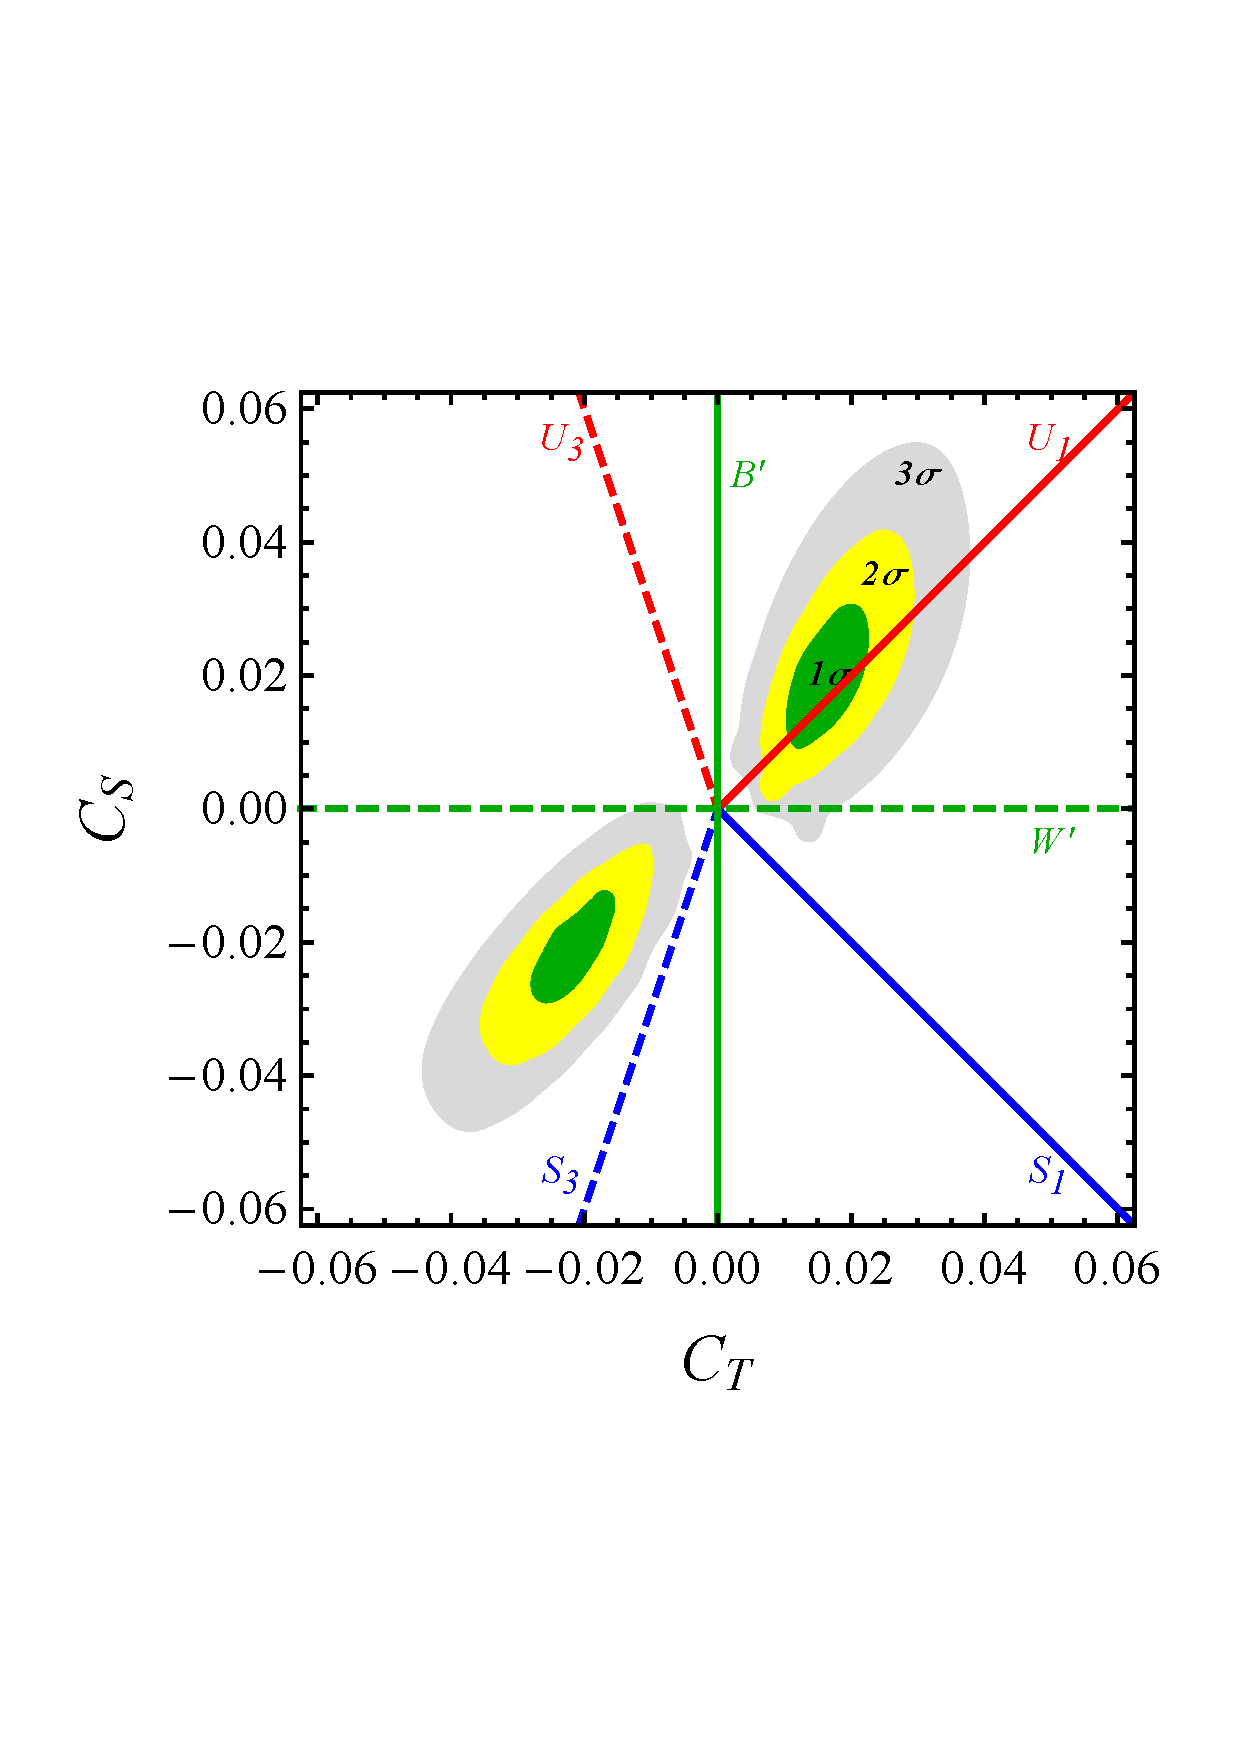
\includegraphics[width=0.75\textwidth]{SMS_fit.pdf} 
      \vspace*{-30mm}
   \caption{Fit of the coefficients $C_T$ and $C_S$ in Eq. \ref{eq:leff} from flavour physics observables. 
   	The parameters $\lambda^q_{sb}$ and  $\lambda^l_{\mu\mu}$ have been marginalised over. 
   	The green, yellow, and grey regions show the 1, 2, and 3$\sigma$ contours, respectively. 
   	Also shown as the straight lines are the correlations between $C_T$ and $C_S$, as predicted in various simplified models with a single mediator: colour-less vectors are shown in green, coloured scalars in blue, and coloured vectors in red. 
   	Electroweak singlet mediators are shown as solid lines, triplets as dashed lines. 
   	From \citep{Buttazzo:2017ixm}.}
\label{fig:fit}
\end{center}
\end{figure}

% =======
\subsection{Simplified Models}
\label{sec:B-SimMod}

The allowed regions in $C_T$ and $C_S$ from the EFT results are not
transparent in terms of an underlying physics idea. However,
they can both be
interpreted as new interactions in a \emph{Stage 3} SM-EFT and can be related
to elements of the concrete BSM models of Sect.~\ref{sec:B-con-BSM} in
a simplified model approach.  As discussed in Sect.~\ref{sec:SimpMod},
the idea of simplified models is to focus on just part of a BSM model, say a
single type of particle and evaluate its constraints and potential
consequences. This approach starts from a Lagrangian consisting of the
SM and a term representing a hypothetical new particle with a free
coupling strength.  The outcome of this Lagrangian is then matched to
Eq.~\ref{eq:leff}.
% The four-fermion operators in Eq. (\ref{eq:leff}) are induced by the exchange of a new heavy particle. 
Assuming $B'(1,1,0)$ or $W'(1,3,0)$; (colour-triplet scalar particles)
$S_1(\bar{3},1,1/3)$ or $S_3(\bar{3},3,1/3)$; (colour-triplet vector
particles), $U_1^\mu(3,1,2/3)$ or $U_3^\mu(3,3,2/3)$\footnote{The
  numbers in brackets indicate the colour, weak, and hypercharge
  quantum numbers.}, one obtains a certain correlation between $C_T$
and $C_S$, shown as straight lines in Fig.~\ref{fig:fit}.  While in
these simplified forms the particles are only defined by their quantum
numbers, they could be interpreted as new electroweak bosons, scalar
or vector leptoquarks, which already were discussed in the context of
concrete BSM models.  Comparing the analysis performed within the
EFT, and the predictions of the different
simplified models, the model with a coloured vector mediator,
$U_1^\mu(3,1,2/3)$, is clearly preferred. 

